% !TEX program = pdflatex
%==============================================================================
%  Rapport de Projet de Fin de Module — Développement Web avec Django
%  E-Shop Django : développement, sécurisation et déploiement d'une
%  plateforme e-commerce moderne (boutique de chaussures)
%  Compilation : pdflatex rapport.tex  (deux passes pour la table des matières)
%==============================================================================
\documentclass[11pt,a4paper]{report}

\usepackage[utf8]{inputenc}
\usepackage[T1]{fontenc}
\usepackage[french]{babel}
\usepackage{lmodern}
\usepackage[a4paper,margin=2.5cm]{geometry}
\usepackage{graphicx}
\usepackage{xcolor}
\usepackage{booktabs}
\usepackage{tabularx}
\usepackage{enumitem}
\usepackage{multicol}
\usepackage{fancyhdr}
\usepackage{titlesec}
\usepackage{listings}
\usepackage{tikz}
\usetikzlibrary{shapes.geometric,arrows.meta,positioning,fit,backgrounds}
\usepackage[hidelinks]{hyperref}
\usepackage{caption}

%--- Couleurs de la charte ----------------------------------------------------
\definecolor{eshopviolet}{RGB}{124,58,237}
\definecolor{eshoppink}{RGB}{219,39,119}
\definecolor{darkgray}{RGB}{45,45,55}
\definecolor{codebg}{RGB}{245,245,250}
\definecolor{codekw}{RGB}{124,58,237}
\definecolor{codestr}{RGB}{16,122,90}
\definecolor{codecom}{RGB}{120,120,135}

%--- En-têtes / pieds de page -------------------------------------------------
\pagestyle{fancy}
\fancyhf{}
\renewcommand{\headrulewidth}{0.4pt}
\fancyhead[L]{\small\itshape E-Shop Django}
\fancyhead[R]{\small\itshape Projet de fin de module — 2025/2026}
\fancyfoot[C]{\thepage}

%--- Style des titres ---------------------------------------------------------
\titleformat{\chapter}[display]
  {\normalfont\huge\bfseries\color{eshopviolet}}
  {\chaptertitlename\ \thechapter}{12pt}{\Huge}
\titlespacing*{\chapter}{0pt}{-10pt}{20pt}

%--- Style du code ------------------------------------------------------------
\lstset{
  basicstyle=\ttfamily\footnotesize,
  backgroundcolor=\color{codebg},
  keywordstyle=\color{codekw}\bfseries,
  stringstyle=\color{codestr},
  commentstyle=\color{codecom}\itshape,
  numberstyle=\tiny\color{codecom},
  numbers=left,
  numbersep=8pt,
  frame=single,
  rulecolor=\color{gray!40},
  breaklines=true,
  showstringspaces=false,
  tabsize=2,
  captionpos=b,
  xleftmargin=14pt,
}

%--- Boîte « encadré » --------------------------------------------------------
\newcommand{\encadre}[2]{%
  \begin{center}
  \fcolorbox{eshopviolet}{eshopviolet!6}{%
    \begin{minipage}{0.94\linewidth}
      \vspace{4pt}
      {\bfseries\color{eshopviolet} #1}\\[2pt]
      #2
      \vspace{4pt}
    \end{minipage}}
  \end{center}
}

\captionsetup{font=small,labelfont={bf,color=eshopviolet}}

%==============================================================================
\begin{document}

%------------------------------------------------------------------ PAGE DE GARDE
\begin{titlepage}
\centering
\vspace*{1cm}

{\scshape\large Génie MIS}\\[0.3cm]
{\scshape Module : Développement Web avec Django}\\[1.2cm]

\rule{\linewidth}{0.4pt}\\[0.4cm]
{\Huge\bfseries\color{eshopviolet} E-Shop Django}\\[0.5cm]
{\LARGE Développement, sécurisation et déploiement\\ d'une plateforme e-commerce moderne}\\[0.4cm]
\rule{\linewidth}{0.4pt}\\[1.0cm]

\begin{tikzpicture}
  \node[rounded corners=10pt, fill=eshopviolet, text=white,
        minimum width=6cm, minimum height=1.6cm, font=\Large\bfseries] {E-Shop $\bullet$ Django};
\end{tikzpicture}

\vfill

\begin{tabular}{rl}


  \textbf{Fait par } & Ali Bouhamidi   -   
Said Aghrod \\[2pt]
  \textbf{Encadré par } & Prof. Bousselham \\
\end{tabular}

\vspace{1cm}
{\large Année universitaire : \textbf{2025 -- 2026}}

\end{titlepage}

%------------------------------------------------------------------ SOMMAIRE
\tableofcontents
\thispagestyle{fancy}

%==============================================================================
\chapter{Introduction générale}
%==============================================================================

Le commerce électronique occupe aujourd'hui une place centrale dans l'économie
mondiale. Les consommateurs achètent en ligne des produits de toutes natures, et
les entreprises s'appuient sur des plateformes web pour présenter leur catalogue,
gérer les commandes, suivre leurs clients et analyser leurs ventes. Maîtriser la
conception d'une telle plateforme constitue donc une compétence essentielle pour
un ingénieur en développement web.

Ce rapport présente \textbf{E-Shop Django}, une plateforme e-commerce complète
développée dans le cadre du projet de fin de module \emph{Développement Web avec
Django}. Le domaine de vente retenu est la \textbf{boutique de chaussures} : le
catalogue, alimenté à partir d'un jeu de données réel (dataset \emph{Myntra},
fichier \texttt{fashion.csv}, sous-catégorie \emph{Shoes}), est organisé par
\textbf{type de chaussure} (décontractées, sport, talons, ballerines, ville) et
séparé en deux rayons \textbf{Homme} et \textbf{Femme}.

L'objectif n'est pas de réaliser un simple site vitrine, mais une
\textbf{application web professionnelle} intégrant la gestion des utilisateurs et
de leurs rôles, un catalogue de produits, un panier d'achat, un processus de
commande, un tableau de bord d'administration, une fonctionnalité
d'\textbf{intelligence artificielle} (recommandation de produits), ainsi que la
\textbf{sécurité}, la \textbf{conteneurisation} et le \textbf{déploiement}
automatisé via une pipeline CI/CD.

%==============================================================================
\chapter{Contexte et problématique}
%==============================================================================

\section{Contexte du projet}
Le développement d'une plateforme e-commerce représente un cas pratique idéal
pour mettre en œuvre les concepts fondamentaux du développement web moderne :
conception d'une application multi-modules, modélisation d'une base de données
relationnelle, authentification et gestion des rôles, développement des
fonctionnalités métier, gestion des fichiers médias, sécurité web, intégration
d'une brique d'intelligence artificielle, conteneurisation avec Docker et mise en
place d'une chaîne d'intégration et de déploiement continus (CI/CD).

\section{Problématique}
\encadre{Problématique}{Comment concevoir, développer, sécuriser et déployer une
plateforme e-commerce moderne avec Django, tout en intégrant une fonctionnalité
intelligente permettant d'améliorer l'expérience utilisateur ?}

Le projet doit en particulier répondre aux questions suivantes :
\begin{itemize}[leftmargin=1.4em]
  \item comment organiser une application Django en plusieurs modules cohérents ?
  \item comment gérer les produits, les catégories, les clients et les commandes ?
  \item comment sécuriser les accès selon les rôles des utilisateurs ?
  \item comment gérer un panier d'achat et le processus de commande ?
  \item comment intégrer une fonctionnalité d'intelligence artificielle utile ?
  \item comment préparer l'application pour un déploiement réel et automatiser sa
        livraison ?
\end{itemize}

%==============================================================================
\chapter{Objectifs}
%==============================================================================

\section{Objectif général}
Développer une plateforme e-commerce générique avec Django permettant à des
utilisateurs de consulter des produits, de gérer un panier, de passer des
commandes et de bénéficier d'une fonctionnalité intelligente de recommandation.

\section{Objectifs spécifiques}
À l'issue du projet, les compétences suivantes ont été mises en œuvre :
\begin{multicols}{2}
\begin{itemize}[leftmargin=1.2em]
  \item concevoir une architecture Django modulaire ;
  \item créer et manipuler des modèles Django ;
  \item gérer une base de données PostgreSQL ;
  \item développer des interfaces avec les templates Django + Bootstrap ;
  \item gérer inscription, connexion et profils ;
  \item développer un catalogue de produits ;
  \item mettre en place un panier d'achat ;
  \item gérer les commandes et leur statut ;
  \item créer un tableau de bord administrateur ;
  \item intégrer une fonctionnalité d'IA ;
  \item sécuriser l'application ;
  \item conteneuriser le projet avec Docker ;
  \item orchestrer les services avec Docker Compose ;
  \item mettre en place une pipeline CI/CD avec GitHub Actions.
\end{itemize}
\end{multicols}

%==============================================================================
\chapter{Analyse des besoins}
%==============================================================================

\section{Acteurs de l'application}
L'application gère trois types d'utilisateurs.

\begin{description}[leftmargin=2.2em,style=nextline]
  \item[Visiteur] Utilisateur non authentifié. Il consulte la page d'accueil et
    le catalogue, recherche et filtre les produits, consulte le détail d'un
    produit et peut créer un compte client.
  \item[Client] Utilisateur authentifié. Il se connecte, modifie son profil,
    ajoute des produits au panier, modifie les quantités, valide une commande,
    consulte l'historique et le statut de ses commandes et laisse des avis.
  \item[Administrateur / gestionnaire] Responsable de la plateforme. Il gère les
    produits, les catégories et les stocks, consulte et fait évoluer le statut
    des commandes, consulte la liste des clients et accède aux statistiques.
\end{description}

\section{Besoins fonctionnels}
\begin{itemize}[leftmargin=1.4em]
  \item \textbf{Gestion des produits} : nom, genre, description, prix, image,
        catégorie, stock, disponibilité, date d'ajout et note moyenne ;
  \item \textbf{Gestion des catégories} : organisation des produits par type ;
  \item \textbf{Catalogue} : grille, recherche par mot-clé, filtre par catégorie
        et par genre, tri (prix, date, nom), pagination ;
  \item \textbf{Panier} : ajout, modification de quantité, suppression, vidage,
        calcul du total ;
  \item \textbf{Commandes} : validation (checkout), statut, historique,
        décrément du stock ;
  \item \textbf{Avis clients} : note (1 à 5 étoiles) et commentaire ;
  \item \textbf{Tableau de bord} : indicateurs clés et statistiques de vente ;
  \item \textbf{Recommandation IA} : suggestion de produits similaires.
\end{itemize}

\section{Besoins non fonctionnels}
Sécurité (authentification, CSRF, contrôle des rôles), performance (requêtes
optimisées, mise en cache du modèle IA, pagination), portabilité
(conteneurisation Docker), maintenabilité (architecture modulaire, tests
automatisés) et ergonomie (interface responsive Bootstrap 5).

%==============================================================================
\chapter{Conception}
%==============================================================================

\section{Diagramme de cas d'utilisation}
La figure~\ref{fig:usecase} présente les principaux cas d'utilisation de la
plateforme, regroupés par acteur. Le client hérite des cas du visiteur
(\emph{generalisation}).

\begin{figure}[ht]
\centering
\begin{tikzpicture}[
  actor/.style={font=\small},
  usecase/.style={draw=eshopviolet, fill=eshopviolet!8, ellipse,
    minimum width=3.1cm, minimum height=0.85cm, align=center, font=\scriptsize},
  every node/.style={transform shape},
  >={Stealth[length=2mm]},
  ]
  % Acteurs
  \node[actor] (visiteur) at (0,3) {\textbf{Visiteur}};
  \node[actor] (client)   at (0,-1.2) {\textbf{Client}};
  \node[actor] (admin)    at (12,1) {\textbf{Admin /}\\ \textbf{gestionnaire}};

  % Cadre système
  \begin{scope}[on background layer]
    \node[draw=gray!50, rounded corners, fill=gray!3, minimum width=8.4cm,
          minimum height=8.6cm] (sys) at (6,1) {};
  \end{scope}
  \node[font=\small\bfseries, anchor=north] at (6,5.2) {Plateforme E-Shop};

  % Cas d'utilisation (visiteur)
  \node[usecase] (cons)  at (6,4.3) {Consulter le catalogue};
  \node[usecase] (rech)  at (6,3.3) {Rechercher / filtrer};
  \node[usecase] (det)   at (6,2.3) {Voir le détail produit};
  \node[usecase] (insc)  at (6,1.3) {Créer un compte};
  % Cas client
  \node[usecase] (pan)   at (6,0.3) {Gérer le panier};
  \node[usecase] (cmd)   at (6,-0.7) {Passer commande};
  \node[usecase] (suivi) at (6,-1.7) {Suivre ses commandes};
  \node[usecase] (avis)  at (6,-2.7) {Laisser un avis};
  % Cas admin
  \node[usecase] (gprod) at (6,-3.6) {Gérer produits / stock};
  \node[usecase] (gcmd)  at (9.2,-2.7) {Gérer les commandes};
  \node[usecase] (stat)  at (9.2,-3.6) {Consulter les statistiques};

  % Liens visiteur
  \draw (visiteur) -- (cons);
  \draw (visiteur) -- (rech);
  \draw (visiteur) -- (det);
  \draw (visiteur) -- (insc);
  % Héritage client -> visiteur
  \draw[->, dashed] (client) -- node[right,font=\tiny]{} (visiteur);
  % Liens client
  \draw (client) -- (pan);
  \draw (client) -- (cmd);
  \draw (client) -- (suivi);
  \draw (client) -- (avis);
  % Liens admin
  \draw (admin) -- (gprod);
  \draw (admin) -- (gcmd);
  \draw (admin) -- (stat);
\end{tikzpicture}
\caption{Diagramme de cas d'utilisation de la plateforme E-Shop.}
\label{fig:usecase}
\end{figure}

\section{Diagramme de classes}
La figure~\ref{fig:class} présente le modèle de classes métier. Les entités
\texttt{Cart}/\texttt{CartItem} et \texttt{Order}/\texttt{OrderItem} suivent le
patron \emph{en-tête / lignes}. Le \texttt{User} natif de Django est étendu par un
\texttt{Profile} (relation 1--1).

\begin{figure}[ht]
\centering
\scalebox{0.86}{
\begin{tikzpicture}[
  class/.style={draw=eshopviolet, fill=white, rectangle, align=left,
    font=\scriptsize\ttfamily, inner sep=4pt},
  title/.style={font=\scriptsize\bfseries},
  >={Stealth[length=2mm]},
  rel/.style={->, >=Stealth},
  ]

  \node[class] (cat) at (0,0) {%
    \textbf{Category}\\\hline
    name\\ slug\\ description\\ created\_at};
  \node[class] (prod) at (4.5,0) {%
    \textbf{Product}\\\hline
    name, gender\\ slug, description\\ price, image\\ stock, available\\ created\_at};
  \node[class] (rev) at (9,0.2) {%
    \textbf{Review}\\\hline
    rating (1--5)\\ comment\\ created\_at};

  \node[class] (user) at (0,-4) {%
    \textbf{User} (Django)\\\hline
    username\\ email\\ password (hashé)\\ is\_staff};
  \node[class] (prof) at (0,-7) {%
    \textbf{Profile}\\\hline
    phone, address\\ city, postal\_code};

  \node[class] (cart) at (4.5,-4) {%
    \textbf{Cart}\\\hline
    user (1--1)\\ created\_at};
  \node[class] (citem) at (4.5,-6.6) {%
    \textbf{CartItem}\\\hline
    quantity\\ subtotal};

  \node[class] (order) at (9,-4) {%
    \textbf{Order}\\\hline
    full\_name, address\\ city, phone\\ status\\ created\_at};
  \node[class] (oitem) at (9,-6.8) {%
    \textbf{OrderItem}\\\hline
    product\_name\\ price, quantity\\ subtotal};

  % Relations
  \draw[rel] (prod) -- node[above,font=\tiny]{*\,--\,1} (cat);
  \draw[rel] (rev)  -- node[above,font=\tiny]{*\,--\,1} (prod);
  \draw[rel] (rev.south) to[bend left=10] node[right,font=\tiny]{*--1} (user.east);
  \draw[rel] (prof) -- node[right,font=\tiny]{1--1} (user);
  \draw[rel] (cart) -- node[above,font=\tiny]{1--1} (user);
  \draw[rel] (citem) -- node[right,font=\tiny]{*--1} (cart);
  \draw[rel] (citem.east) to[bend right=20] node[below,font=\tiny]{*--1} (prod.south);
  \draw[rel] (order) -- node[right,font=\tiny]{*--1} (user.east);
  \draw[rel] (oitem) -- node[right,font=\tiny]{*--1} (order);
\end{tikzpicture}}
\caption{Diagramme de classes (modèle de données métier).}
\label{fig:class}
\end{figure}

\section{Modèle de données}
\begin{center}
\renewcommand{\arraystretch}{1.25}
\begin{tabularx}{\linewidth}{@{}lX@{}}
\toprule
\textbf{Entité} & \textbf{Description} \\
\midrule
\texttt{User} & Compte (client, gestionnaire ou administrateur), géré par Django. \\
\texttt{Profile} & Informations complémentaires du client (téléphone, adresse). \\
\texttt{Category} & Catégorie / type de chaussure. \\
\texttt{Product} & Produit vendu (nom, genre, prix, image, stock, disponibilité). \\
\texttt{Cart} & Panier persistant d'un client (1 panier par utilisateur). \\
\texttt{CartItem} & Ligne de panier : un produit + une quantité. \\
\texttt{Order} & Commande validée (adresse de livraison, statut). \\
\texttt{OrderItem} & Ligne de commande : nom, prix unitaire et quantité figés. \\
\texttt{Review} & Avis : note (1 à 5) et commentaire, unique par couple client/produit. \\
\bottomrule
\end{tabularx}
\end{center}

%==============================================================================
\chapter{Architecture technique et choix technologiques}
%==============================================================================

\section{Architecture applicative}
Le projet suit une architecture Django modulaire : chaque domaine métier est isolé
dans une \emph{application} Django dédiée, ce qui favorise la séparation des
responsabilités et la maintenabilité.

\begin{lstlisting}[language=bash,caption={Arborescence du projet},captionpos=b]
ecommerce_project/   # configuration : settings, urls, wsgi
accounts/            # utilisateurs, inscription, connexion, profils
products/            # produits, categories, recherche, filtres, avis
cart/                # panier d'achat
orders/              # commandes et checkout
dashboard/           # statistiques et administration
recommendation/      # fonctionnalite IA (TF-IDF + similarite cosinus)
templates/  static/  media/
Dockerfile  docker-compose.yml  nginx/  entrypoint.sh
requirements.txt  .env  .github/workflows/ci-cd.yml
\end{lstlisting}

L'application suit le patron \textbf{MVT} (Model–View–Template) de Django. Un
\emph{context processor} (\texttt{cart.context\_processors.cart\_summary}) injecte
le résumé du panier dans toutes les pages.

\section{Choix technologiques}
\begin{center}
\renewcommand{\arraystretch}{1.25}
\begin{tabularx}{\linewidth}{@{}lX@{}}
\toprule
\textbf{Couche} & \textbf{Technologie retenue} \\
\midrule
Backend & Django 5.0 (Python 3.11) \\
Frontend & Templates Django + Bootstrap 5 + Bootstrap Icons \\
Base de données & PostgreSQL 16 (SQLite en développement local) \\
Authentification & Système d'authentification natif de Django \\
Fichiers médias & Django Media Files (Pillow) \\
Fichiers statiques & WhiteNoise (compression + manifest) \\
Intelligence artificielle & scikit-learn — TF-IDF + similarité cosinus \\
Tests & Django \texttt{TestCase} \\
Serveur d'application & Gunicorn (3 workers WSGI) \\
Reverse proxy & Nginx \\
Conteneurisation & Docker \& Docker Compose \\
CI/CD & GitHub Actions \\
Registre d'images & GitHub Container Registry (GHCR) \\
\bottomrule
\end{tabularx}
\end{center}

Les dépendances Python principales (\texttt{requirements.txt}) sont :
\texttt{Django}, \texttt{psycopg2-binary}, \texttt{python-dotenv}, \texttt{Pillow},
\texttt{gunicorn}, \texttt{whitenoise}, \texttt{dj-database-url} et
\texttt{scikit-learn}.

%==============================================================================
\chapter{Description des fonctionnalités}
%==============================================================================

\section{Comptes et gestion des rôles}
L'inscription crée un compte et connecte automatiquement le nouvel utilisateur ; un
\texttt{Profile} est généré par un signal \texttt{post\_save}. Le client peut
modifier son profil. Trois rôles coexistent : visiteur, client (\texttt{User}
authentifié) et administrateur / gestionnaire (\texttt{is\_staff}).

\section{Catalogue, recherche et filtres}
La vue \texttt{product\_list} combine recherche plein texte (sur le nom et la
description), filtre par catégorie, filtre par genre (\texttt{?gender=Men|Women}),
tri (prix croissant/dé\-croissant, date, nom) et pagination (9 produits par page).
Seuls les produits disponibles sont affichés. La page d'accueil met en avant les
types de chaussures et deux rayons \emph{Homme} et \emph{Femme}
(figures~\ref{fig:hero} et~\ref{fig:homme}).

\section{Panier d'achat}
Le panier est persistant (un \texttt{Cart} par utilisateur). Les opérations
disponibles sont : ajout, mise à jour de la quantité, suppression d'une ligne,
vidage complet et calcul du total. Les quantités sont systématiquement bornées par
le stock disponible.

\section{Commandes et checkout}
La validation (\texttt{checkout}) s'effectue dans une \textbf{transaction
atomique} : vérification du stock de chaque ligne, création de la \texttt{Order} et
des \texttt{OrderItem} (le nom et le prix unitaire sont figés à l'instant de
l'achat), décrément du stock puis vidage du panier. Une commande suit un cycle de
vie à six statuts : \emph{en attente, confirmée, en préparation, expédiée, livrée,
annulée}. Le client consulte l'historique et le détail de ses commandes.

\section{Avis clients}
Un client authentifié note un produit (1 à 5 étoiles) et laisse un commentaire ; la
contrainte \texttt{unique\_together(product, user)} garantit un seul avis par
produit et par client. La note moyenne (\texttt{average\_rating}) et le nombre
d'avis sont calculés par agrégation.

\section{Tableau de bord administrateur}
Réservé aux utilisateurs \texttt{is\_staff} (décorateur
\texttt{user\_passes\_test}), le tableau de bord (figure~\ref{fig:dashboard})
affiche le nombre total de produits, de clients et de commandes, le chiffre
d'affaires (hors commandes annulées), les produits les plus vendus, les commandes
récentes, la répartition des commandes par statut et les alertes de stock faible.
L'interface d'administration Django (figure~\ref{fig:admin}) complète ce dispositif
pour les opérations CRUD.

%==============================================================================
\chapter{Fonctionnalité d'intelligence artificielle}
%==============================================================================

\encadre{Fonctionnalité IA}{Un système de \textbf{recommandation de produits
similaires} basé sur le contenu (\emph{content-based filtering}), affiché sur
chaque fiche produit sous le bloc « Vous aimerez aussi ».}

\section{Principe}
Le moteur (module \texttt{recommendation/}) repose sur deux techniques classiques
du traitement automatique du langage, implémentées avec \textbf{scikit-learn} :
\begin{enumerate}[leftmargin=1.6em]
  \item Chaque produit est transformé en un « document » texte concaténant son
        nom (pondéré), sa catégorie (pondérée) et sa description.
  \item Le vectoriseur \textbf{TF-IDF} est \emph{entraîné} sur un échantillon
        aléatoire de \textbf{20~\%} du catalogue (apprentissage du vocabulaire et
        des poids IDF), en n-grammes (1,2) et avec une liste de mots vides
        français.
  \item L'ensemble du catalogue est ensuite \emph{projeté} (\texttt{transform})
        dans cet espace TF-IDF.
  \item La \textbf{similarité cosinus} entre tous les produits est calculée ; pour
        un produit donné, on retourne les $k$ produits les plus proches (hors
        lui-même et hors score nul).
\end{enumerate}

\section{Optimisation et robustesse}
Le modèle est mis en cache en mémoire : il n'est reconstruit que lorsque la
\emph{signature} du catalogue change (nombre de produits ou date de dernière mise à
jour). Si le moteur ne renvoie aucun résultat, la vue effectue un repli sur les
produits de la même catégorie, garantissant une recommandation pertinente en toute
circonstance.

\begin{lstlisting}[language=Python,caption={Cœur du moteur de recommandation (extrait simplifié)}]
vectorizer = TfidfVectorizer(stop_words=FRENCH_STOP_WORDS,
                             lowercase=True, ngram_range=(1, 2))
vectorizer.fit(train_corpus)            # entrainement sur 20 % des produits
tfidf_matrix = vectorizer.transform(corpus)   # projection du catalogue complet
self._similarity = cosine_similarity(tfidf_matrix)   # matrice de similarite
\end{lstlisting}

%==============================================================================
\chapter{Sécurité}
%==============================================================================

Les bonnes pratiques de sécurité exigées par le cahier des charges sont respectées :
\begin{itemize}[leftmargin=1.4em]
  \item \textbf{Authentification obligatoire} pour le panier, le checkout et les
        avis (décorateur \texttt{@login\_required}) ;
  \item \textbf{mots de passe hachés} par Django et validés par les quatre
        \emph{password validators} activés ;
  \item \textbf{protection CSRF} active et validation des formulaires côté serveur ;
  \item \textbf{contrôle des rôles} : l'espace administrateur et le tableau de bord
        sont protégés par \texttt{is\_staff} ; un client ne peut accéder qu'à ses
        propres commandes ;
  \item \textbf{variables sensibles} (\texttt{SECRET\_KEY}, identifiants de base de
        données) placées dans un fichier \texttt{.env} non versionné ;
  \item \textbf{mode debug désactivé en production} (\texttt{DEBUG=False}), avec
        cookies sécurisés, en-tête \texttt{HSTS}, \texttt{X-Frame-Options: DENY} et
        \texttt{Content-Type nosniff} ;
  \item \textbf{taille des fichiers uploadés limitée} (2,5~Mo) côté Django et 5~Mo
        côté Nginx.
\end{itemize}

\encadre{Attention}{Les mots de passe ne sont jamais stockés en clair et le fichier
\texttt{.env} n'est jamais publié sur GitHub (\texttt{.gitignore}).}

%==============================================================================
\chapter{Déploiement}
%==============================================================================

\section{Conteneurisation}
L'application est empaquetée dans une image Docker basée sur
\texttt{python:3.11-slim}. Un script d'entrée (\texttt{entrypoint.sh}) attend que
PostgreSQL soit prêt, applique les migrations, charge les données initiales si la
base est vide (\texttt{datadump.json} ou import depuis \texttt{fashion.csv}),
collecte les fichiers statiques, puis lance Gunicorn.

\section{Orchestration locale (Docker Compose)}
Le fichier \texttt{docker-compose.yml} orchestre trois services :
\begin{itemize}[leftmargin=1.4em]
  \item \texttt{db} — PostgreSQL 16 avec volume persistant et \emph{healthcheck} ;
  \item \texttt{web} — l'application Django servie par Gunicorn (3 workers) ;
  \item \texttt{nginx} — reverse proxy exposé sur le port 80, servant directement
        les fichiers statiques et médias.
\end{itemize}
Toutes les variables sensibles sont fournies par le fichier \texttt{.env}.

\begin{lstlisting}[language=bash,caption={Démarrage de la stack complète}]
cp .env.example .env        # renseigner DB_NAME, DB_USER, DB_PASSWORD, DB_HOST=db
docker compose up --build   # http://localhost  (Nginx -> Gunicorn -> PostgreSQL)
\end{lstlisting}

\section{Production}
La configuration de production impose \texttt{DEBUG=False}, une
\texttt{SECRET\_KEY} issue de l'environnement, Gunicorn comme serveur WSGI, Nginx
comme reverse proxy, PostgreSQL comme base de données et une gestion correcte des
fichiers statiques (WhiteNoise) et médias. Le projet est déployable sur une machine
virtuelle Ubuntu, un VPS ou une plateforme PaaS (Render, Railway).

%==============================================================================
\chapter{Pipeline CI/CD}
%==============================================================================

\encadre{Objectif}{Automatiser les tests, la vérification de la qualité du code, la
construction de l'image Docker et sa publication à chaque \texttt{push} sur la
branche principale.}

La pipeline GitHub Actions (\texttt{.github/workflows/ci-cd.yml}) se décompose en
deux jobs enchaînés :
\begin{enumerate}[leftmargin=1.6em]
  \item \textbf{Tests \& qualité} — récupération du code, installation de
        Python~3.11 et des dépendances, analyse statique avec \texttt{flake8},
        exécution des migrations puis des tests sur un service PostgreSQL ;
  \item \textbf{Build \& publication} — uniquement sur \texttt{push} vers
        \texttt{main} : connexion à GitHub Container Registry et publication de
        l'image Docker, taguée \texttt{latest} et avec le SHA du commit.
\end{enumerate}

\begin{lstlisting}[language=bash,caption={Extrait du workflow GitHub Actions}]
on:
  push:        { branches: [main] }
  pull_request:{ branches: [main] }
jobs:
  test:           # flake8 + migrate + manage.py test (PostgreSQL)
  build-and-push: # docker build + push -> ghcr.io  (needs: test)
\end{lstlisting}

%==============================================================================
\chapter{Captures d'écran}
%==============================================================================

\begin{figure}[ht]
  \centering
  \fbox{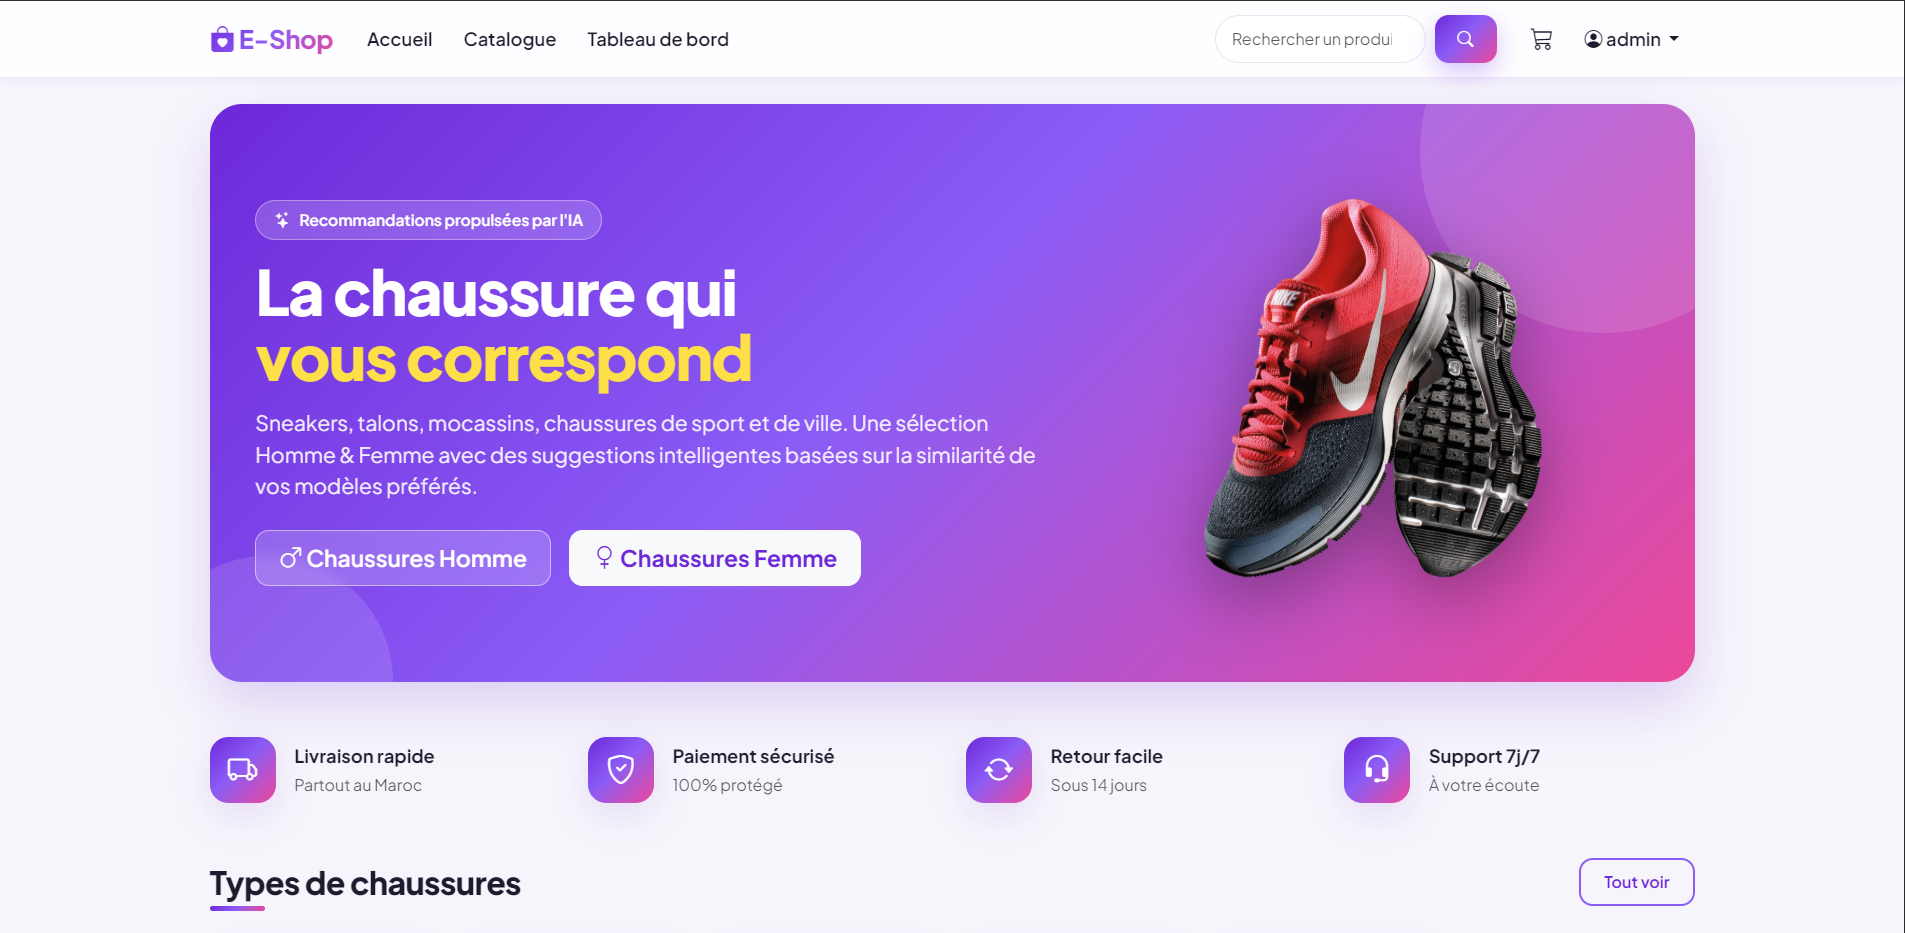
\includegraphics[width=0.95\linewidth]{screenshots/fig-accueil-hero.png}}
  \caption{Page d'accueil — section « hero » et accès aux rayons Homme / Femme,
           avec la mention des recommandations proposées par l'IA.}
  \label{fig:hero}
\end{figure}

\begin{figure}[ht]
  \centering
  \fbox{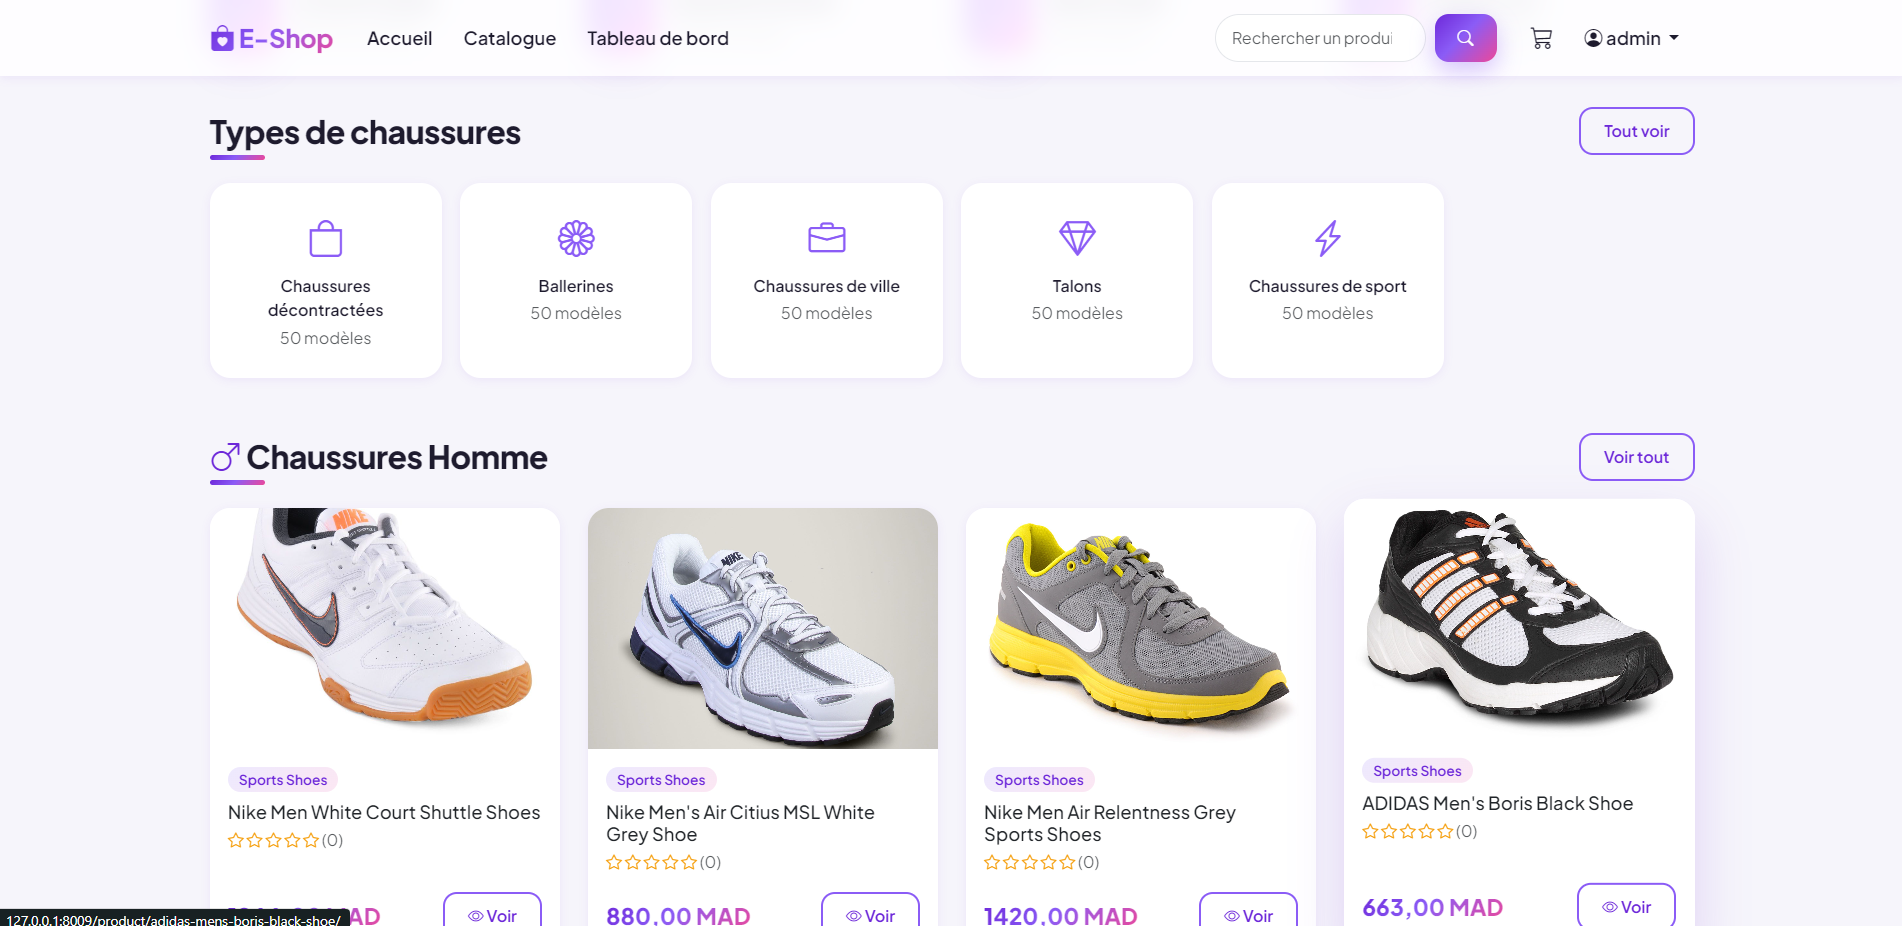
\includegraphics[width=0.95\linewidth]{screenshots/fig-accueil-homme.png}}
  \caption{Page d'accueil — types de chaussures et rayon « Chaussures Homme »
           sous forme de grille de produits (prix en MAD).}
  \label{fig:homme}
\end{figure}

\begin{figure}[ht]
  \centering
  \fbox{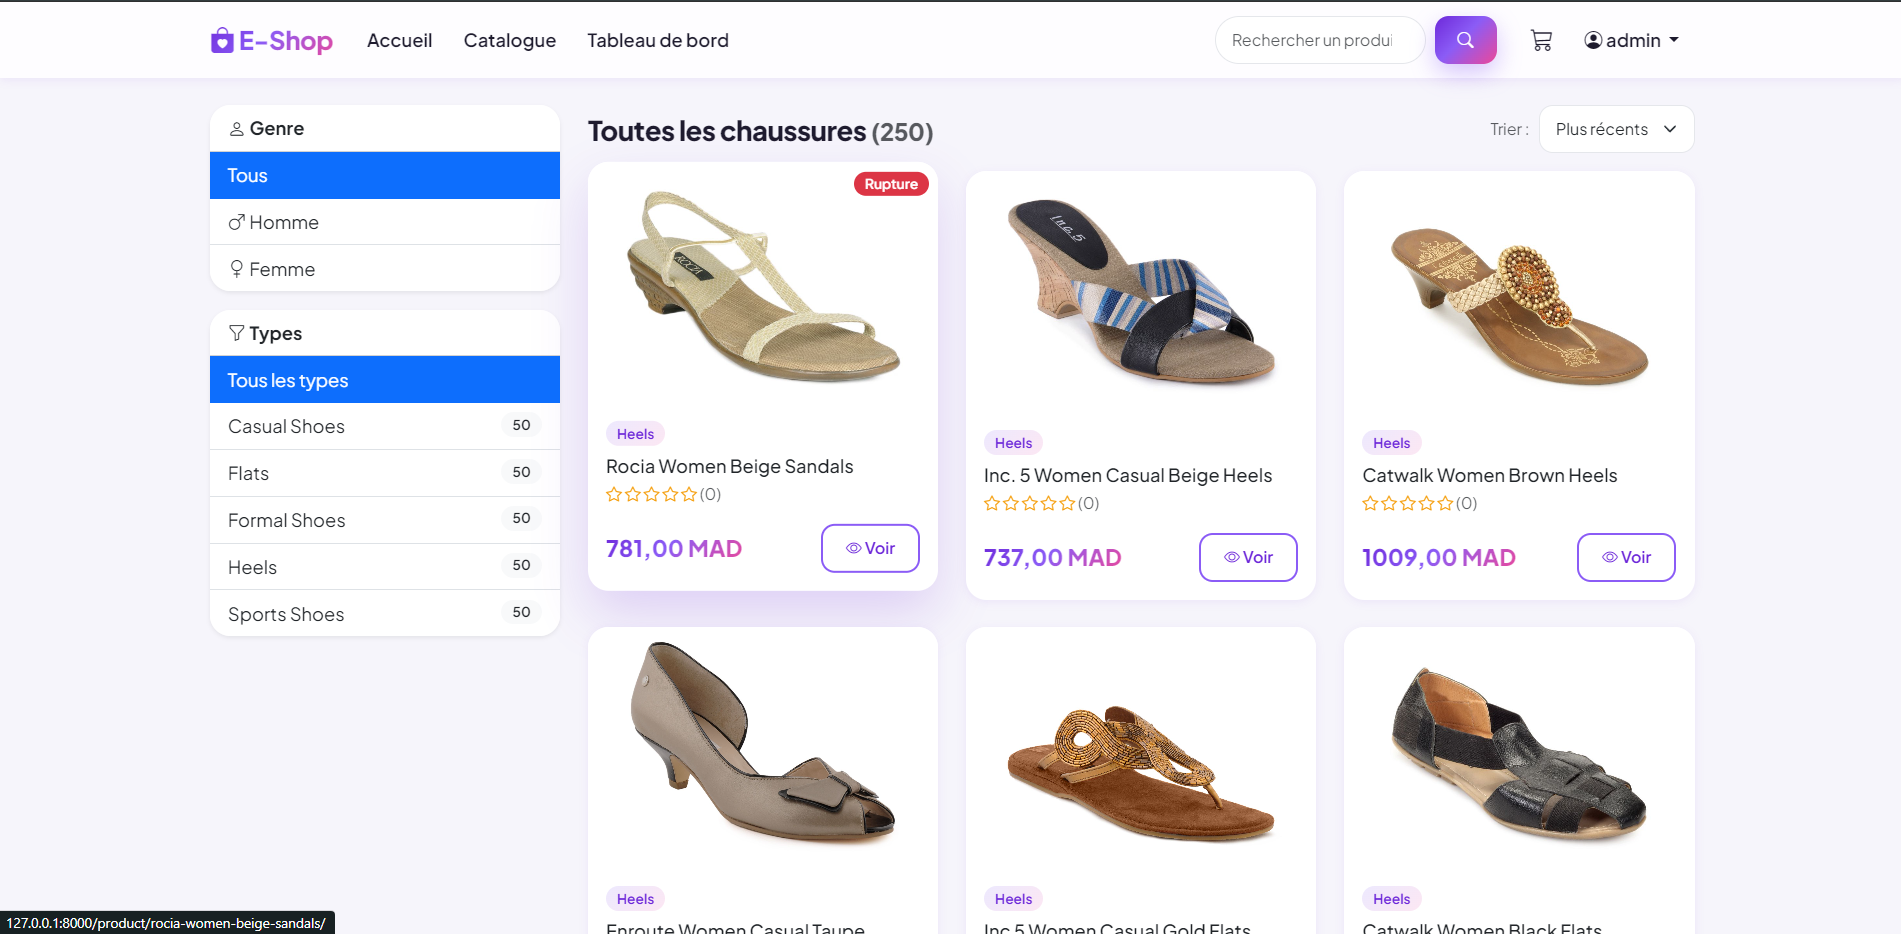
\includegraphics[width=0.95\linewidth]{screenshots/fig-catalogue.png}}
  \caption{Catalogue — grille de produits avec filtres (genre, types) et tri ;
           250 produits disponibles.}
  \label{fig:catalogue}
\end{figure}

\begin{figure}[ht]
  \centering
  \fbox{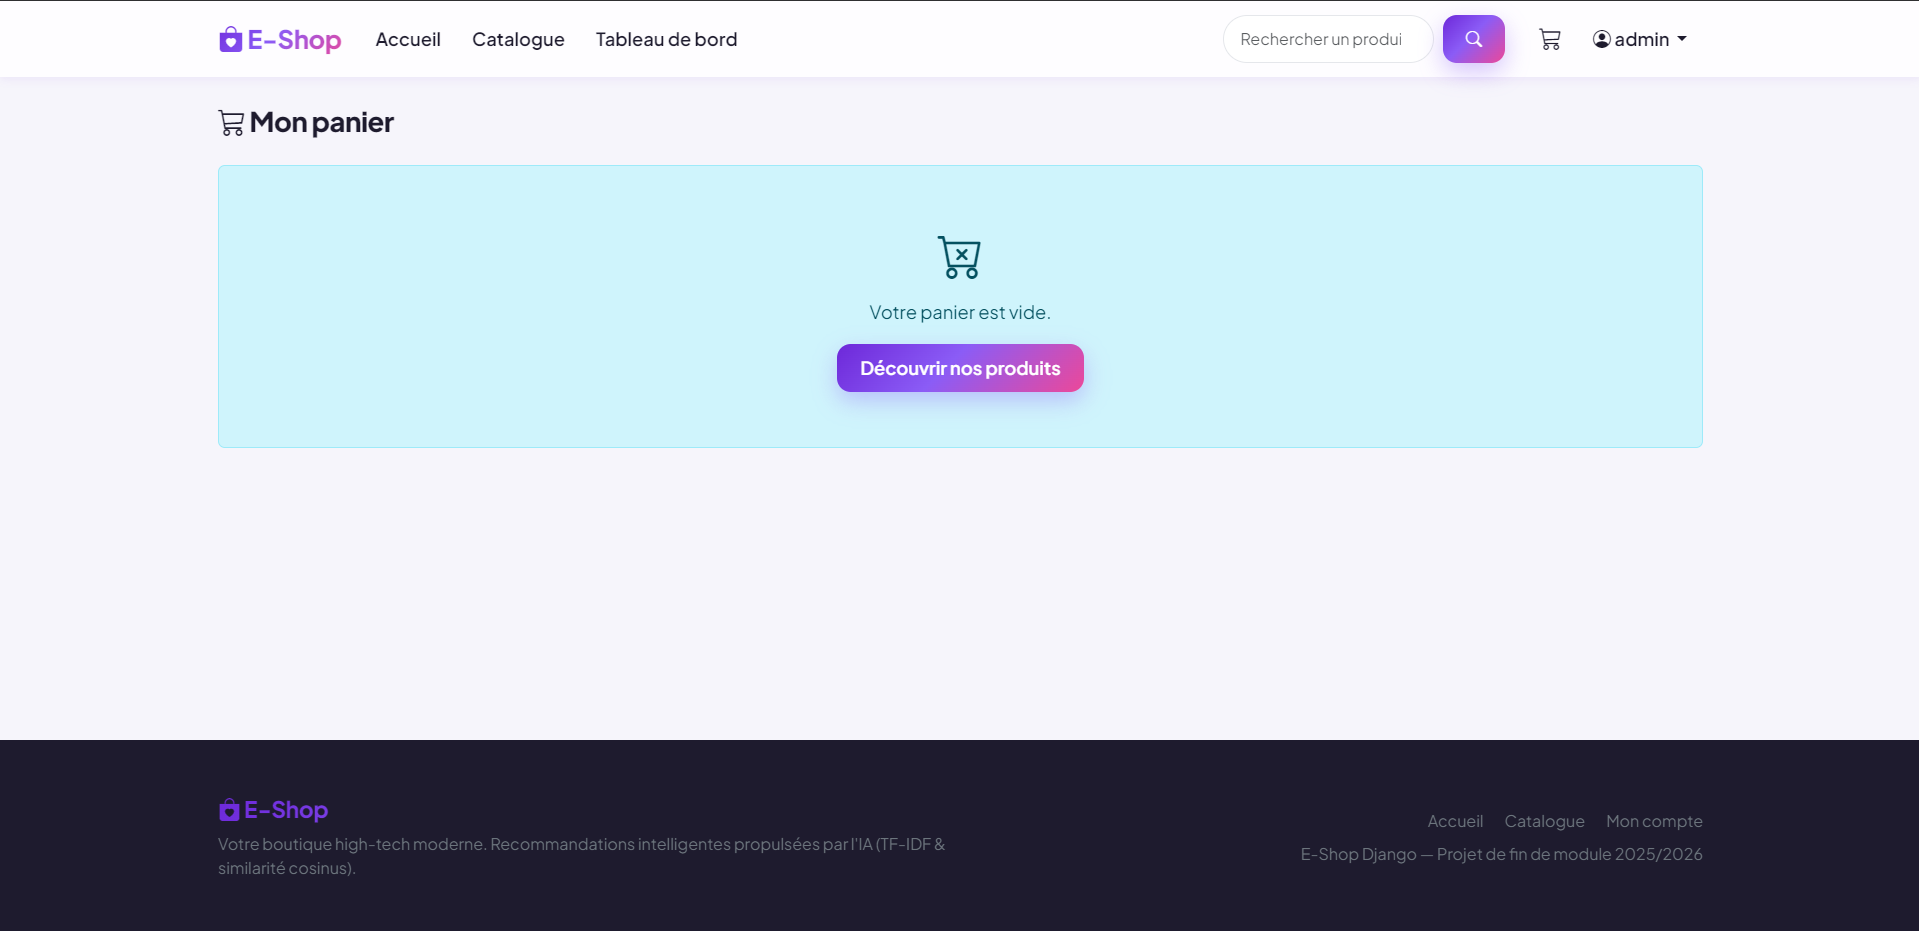
\includegraphics[width=0.95\linewidth]{screenshots/fig-panier.png}}
  \caption{Panier d'achat (ici vide) avec invitation à découvrir les produits.}
  \label{fig:panier}
\end{figure}

\begin{figure}[ht]
  \centering
  \fbox{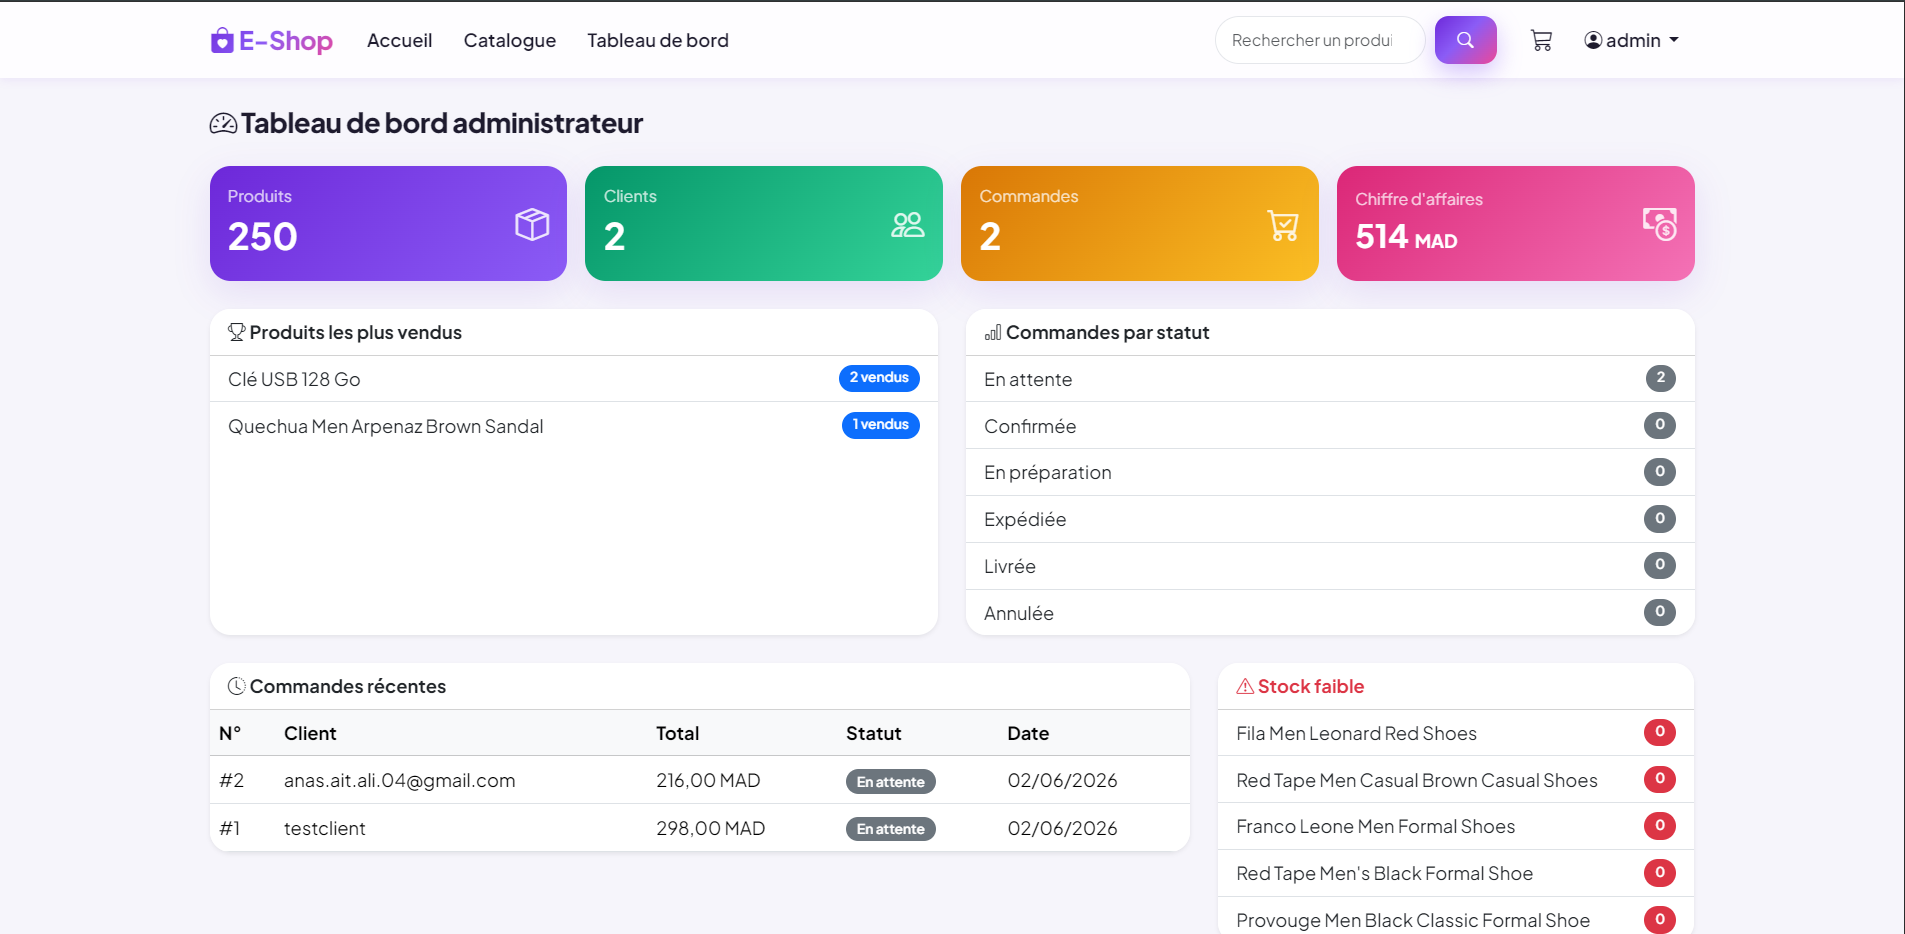
\includegraphics[width=0.95\linewidth]{screenshots/fig-dashboard.png}}
  \caption{Tableau de bord administrateur — indicateurs (produits, clients,
           commandes, chiffre d'affaires), meilleures ventes, commandes par statut,
           commandes récentes et alertes de stock faible.}
  \label{fig:dashboard}
\end{figure}

\begin{figure}[ht]
  \centering
  \fbox{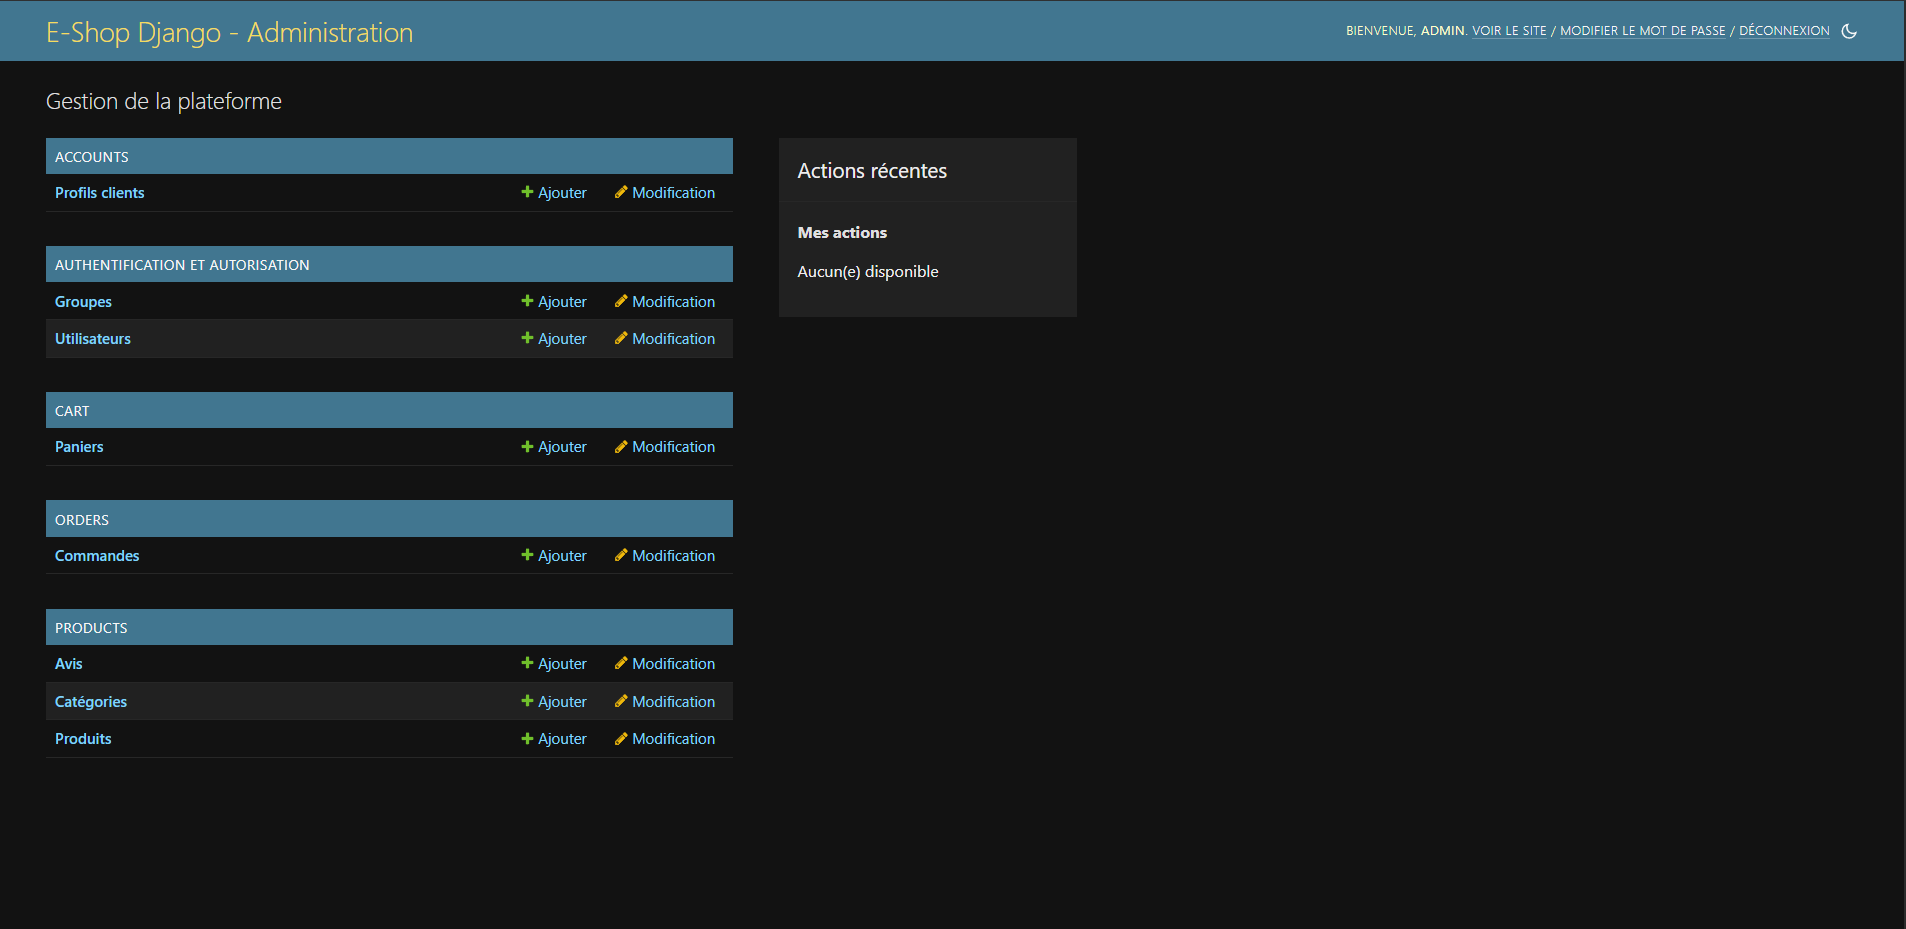
\includegraphics[width=0.95\linewidth]{screenshots/fig-admin.png}}
  \caption{Interface d'administration Django — gestion CRUD des comptes, paniers,
           commandes, catégories, produits et avis.}
  \label{fig:admin}
\end{figure}

\clearpage

%==============================================================================
\chapter{Difficultés rencontrées}
%==============================================================================

\begin{itemize}[leftmargin=1.4em]
  \item \textbf{Données réelles} — l'import et le nettoyage du dataset Myntra
        (\texttt{fashion.csv}) ont nécessité une commande de gestion dédiée
        (\texttt{import\_fashion}) pour structurer les produits par type et par
        genre et associer des images.
  \item \textbf{Recommandation en français} — scikit-learn ne fournissant pas de
        liste de mots vides française, une liste réduite a été constituée
        manuellement ; l'entraînement du TF-IDF sur seulement 20~\% du catalogue
        impose un mécanisme de repli par catégorie.
  \item \textbf{Performance de l'IA} — recalculer la matrice de similarité à chaque
        requête étant coûteux, une mise en cache invalidée par la signature du
        catalogue a été mise en place.
  \item \textbf{Cohérence des commandes} — le décrément du stock et la création des
        lignes de commande ont dû être encapsulés dans une transaction atomique
        avec vérification préalable du stock.
  \item \textbf{Initialisation en conteneur} — l'\texttt{entrypoint} doit attendre
        PostgreSQL, appliquer les migrations et charger les données de façon
        \emph{idempotente} pour éviter tout doublon lors d'un redémarrage.
\end{itemize}

%==============================================================================
\chapter{Conclusion et perspectives}
%==============================================================================

Ce projet a permis de concevoir, développer, sécuriser et déployer une plateforme
e-commerce complète avec Django, répondant à l'ensemble des exigences du cahier des
charges : architecture modulaire, gestion des utilisateurs et des rôles, catalogue,
panier, commandes, avis, tableau de bord, et une fonctionnalité d'intelligence
artificielle de recommandation fondée sur TF-IDF et la similarité cosinus.
L'application est conteneurisée avec Docker, orchestrée par Docker Compose
(Nginx + Gunicorn + PostgreSQL) et livrée automatiquement via une pipeline CI/CD
GitHub Actions.

\paragraph{Perspectives.} Plusieurs évolutions sont envisageables :
\begin{itemize}[leftmargin=1.4em]
  \item une recommandation \textbf{personnalisée} fondée sur l'historique d'achat
        et de navigation de chaque client ;
  \item l'intégration d'un \textbf{paiement en ligne} (Stripe, PayPal) ;
  \item l'exposition d'une \textbf{API REST} (Django REST Framework) pour une
        application mobile ;
  \item l'ajout d'un \textbf{moteur de recherche avancé} et de la gestion des
        promotions ;
  \item un \textbf{déploiement continu} automatique vers un serveur de production,
        complété par des scans de sécurité des dépendances et de l'image Docker.
\end{itemize}

\vfill
\begin{center}\itshape
E-Shop Django — Projet de fin de module 2025/2026.
\end{center}

\end{document}
